\section{Preliminary results}

To ensure that potentiation in NK landscapes is not entirely trivial, I ran some very early preliminary data. 
I selected $N=10$ and enumerated potentiation in 50 landscapes each of $K \in \{0,1,2,3\}$.
For each landscape, I ran 50 replicates from every genotype (1,024 genotypes per landscape) to quantify potentiation at that point. 
%These data are not fully analyzed and these plots are rough, this was last-minute data to make sure this environment was worth looking into. 

\begin{figure}[h!]
    \centering
    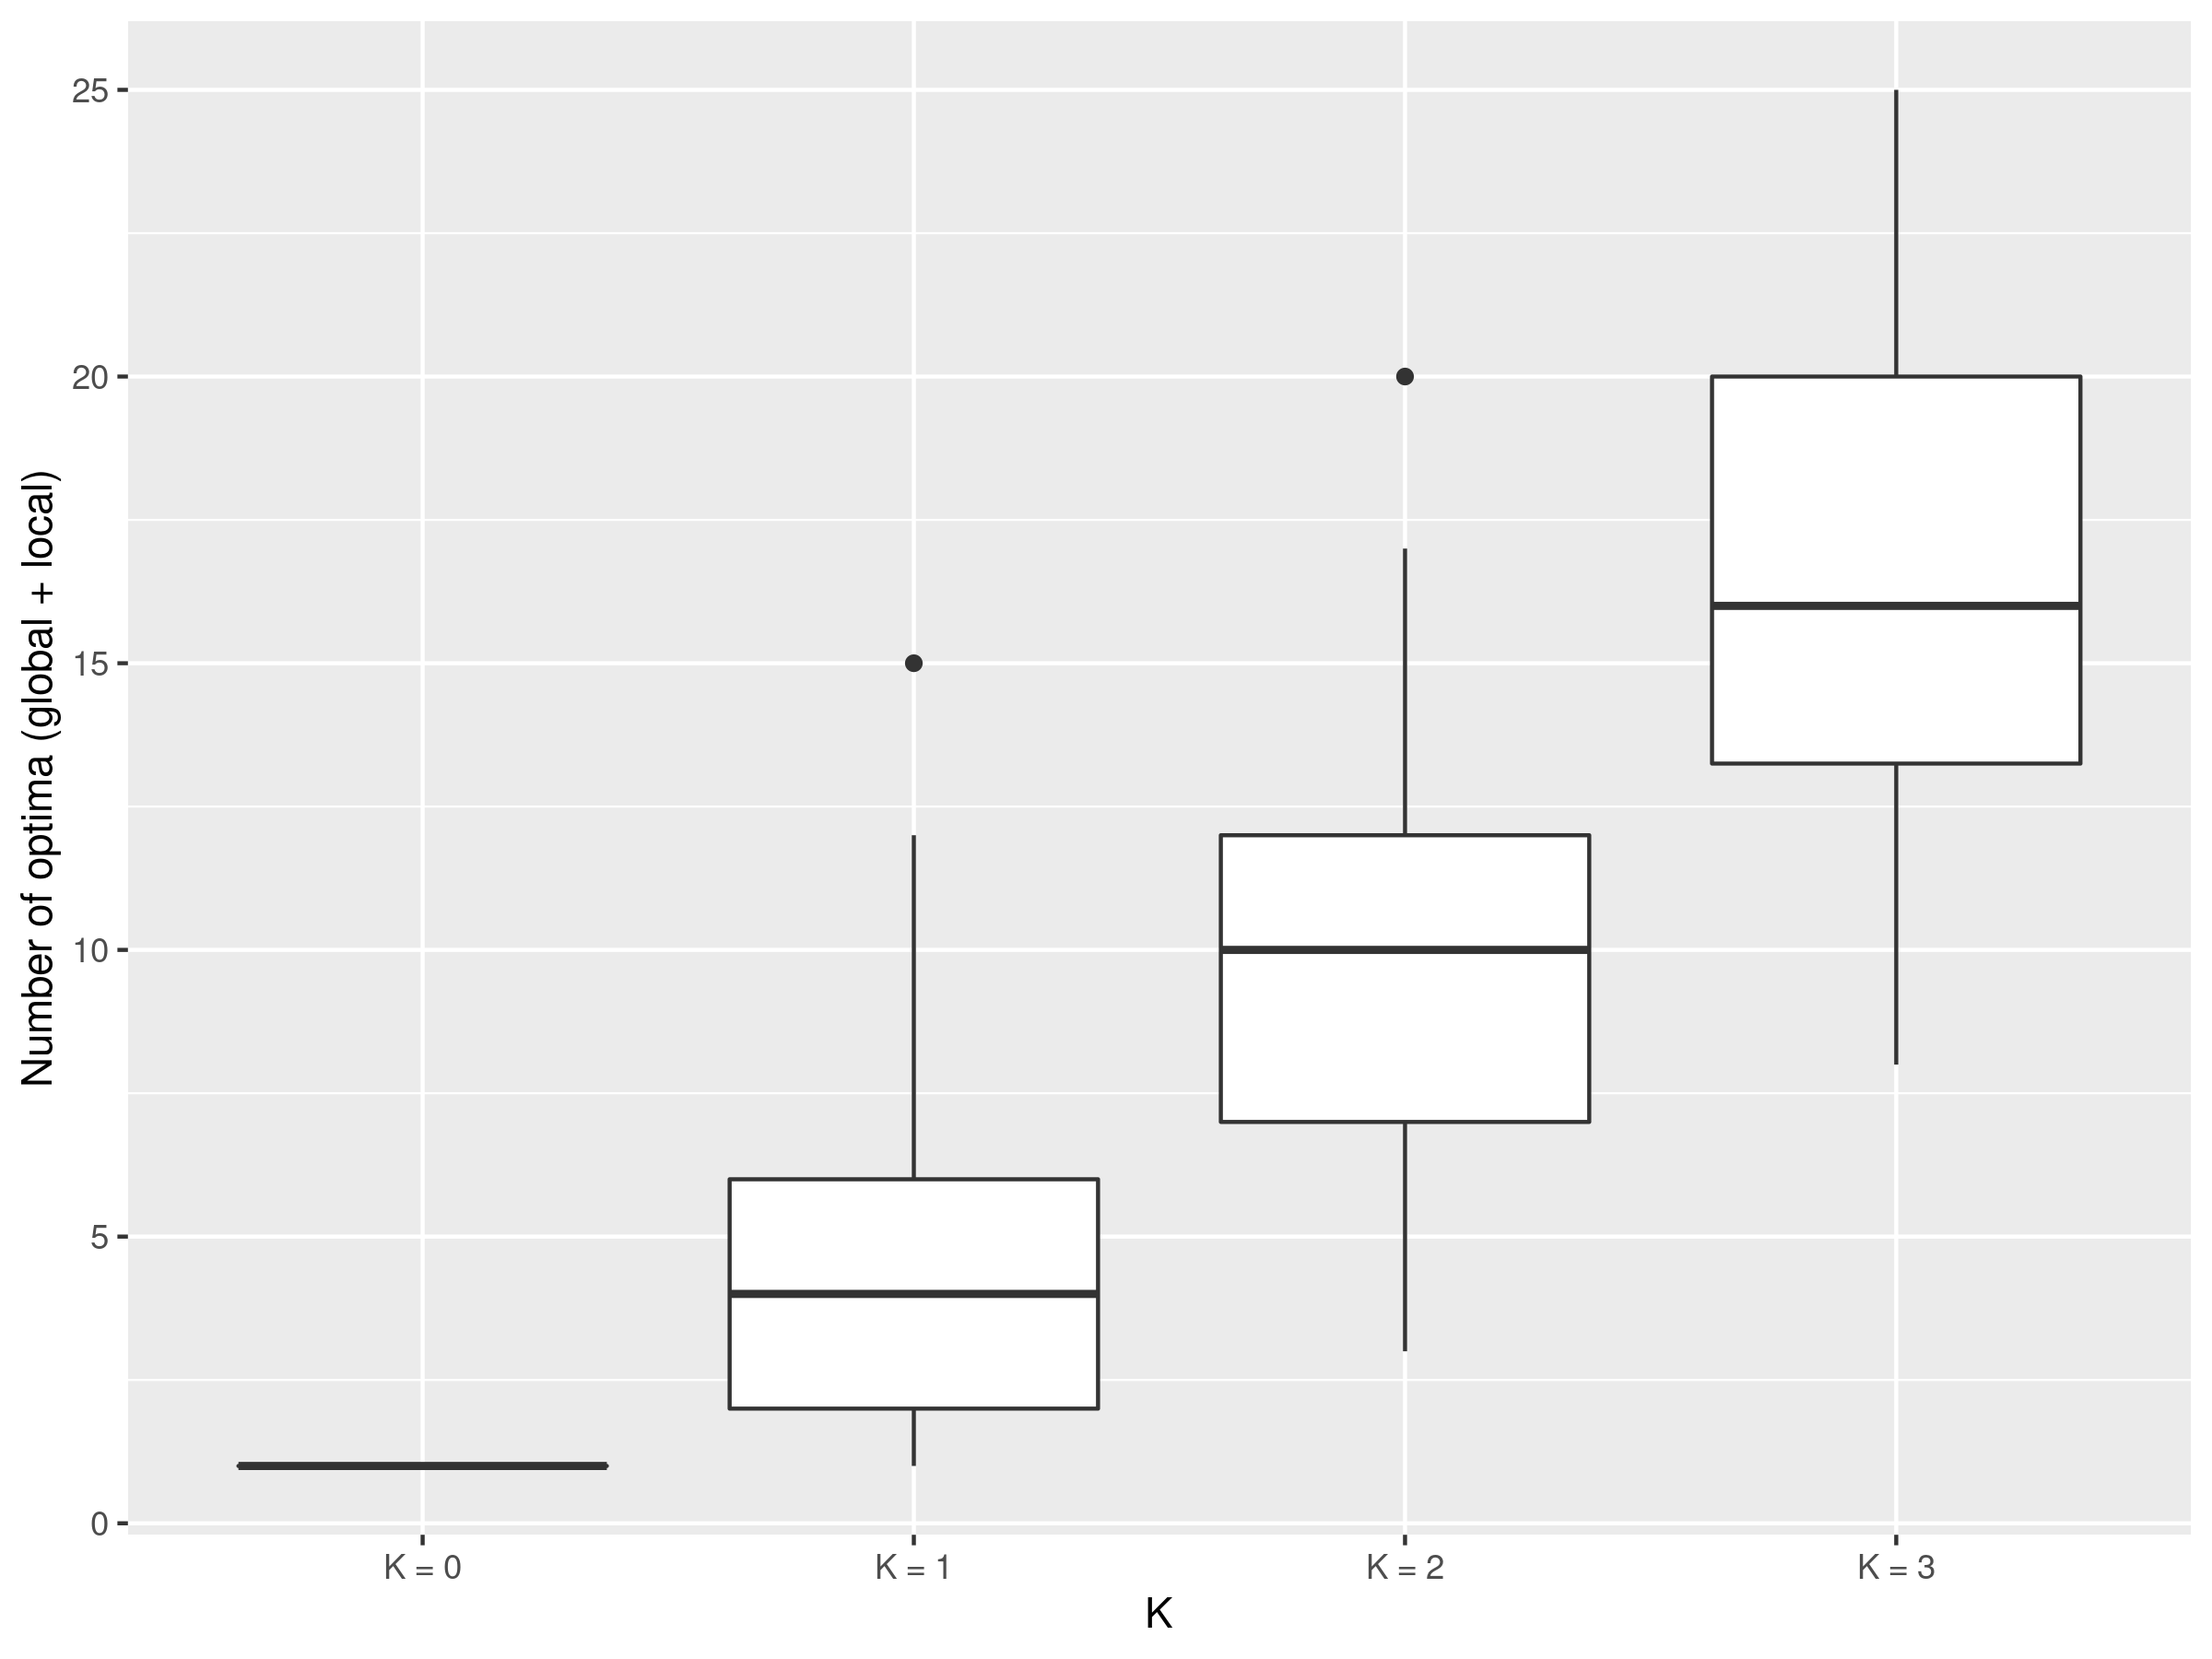
\includegraphics[width=0.95\textwidth]{04_simplified_model/media/num_peaks.png}
    \caption{
        Boxplots showing the number of peaks in all 50 landscapes of a given $K$ value. 
    }
    \label{fig:simplified_model:num_peaks}
\end{figure}

First, Figure \ref{fig:simplified_model:num_peaks} shows the number of peaks at each $K$ value. 
Here we define a peak as a genotype that has higher fitness than the $N$ genotypes around it; this definition includes local optima as well as the global optimum \citep{ostmanPredictingEvolutionVisualizing2014}. 
NK landscapes are often described as ``tunably rugged'', with larger $K$ values creating more rugged landscapes due to increased epistatic interactions. 
We see exactly that here, as the number of peaks increases smoothly as we increase $K$. 

\begin{figure}[h!]
    \centering
    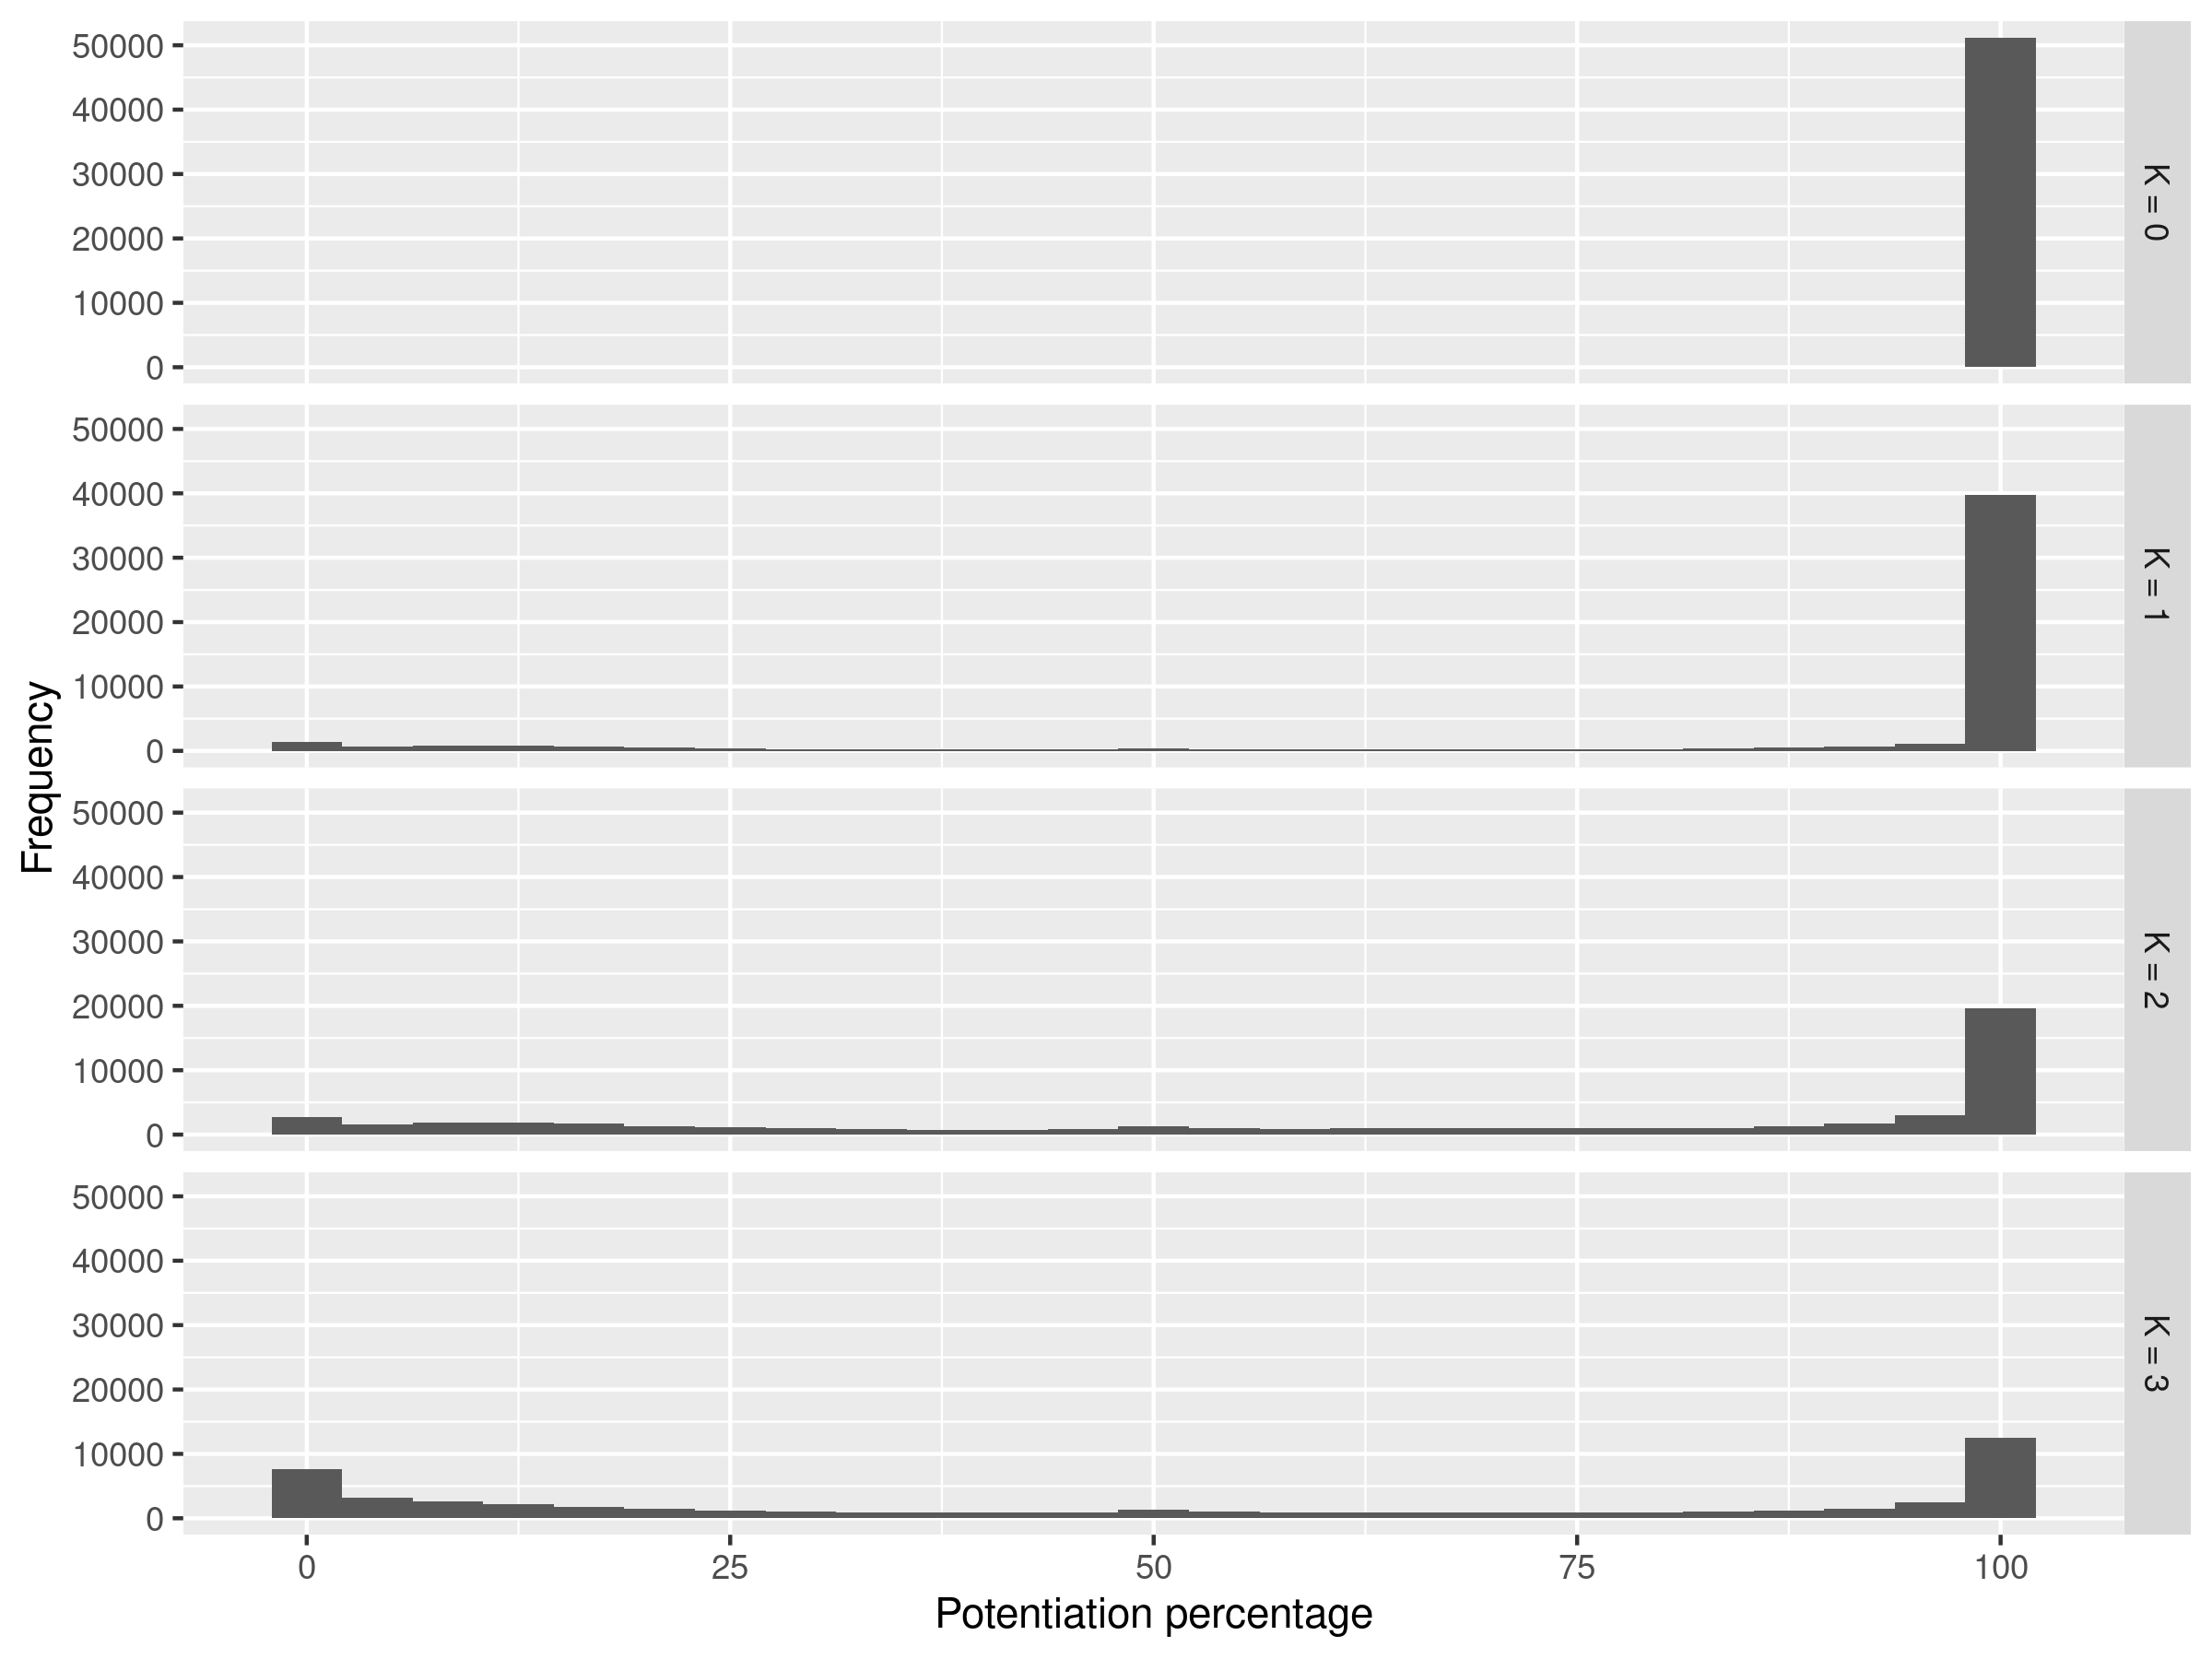
\includegraphics[width=0.95\textwidth]{04_simplified_model/media/success_histogram.png}
    \caption{
        Histograms of potentiation, with one row per $K$ value.
        Each histogram includes the potentiation of all 1,024 genotypes in all 50 landscapes for that $K$ value.
    }
    \label{fig:simplified_model:potentaition_histogram}
\end{figure}

Figure \ref{fig:simplified_model:potentaition_histogram} shows the overall distribution of potentiation across all genotypes in all landscapes at each $K$ value. 
First, $K=0$ shows 100\% potentiation for every genotype in every landscape, which matches expectations as individual bits can be optimized independently (i.e., there is zero epistasis) and thus the landscape is a single hill to climb. 
As $K$ increases, we see some mass of the distribution shift from 100\% potentiation to the lower values, especially the very low values around 0\%. 
This also meets my expectation, as we have shown that increasing $K$ increases the number of local optima and thus creates more opportunities for populations to become ``stuck'' and unable to reach the global optimum. 
When it comes time to compare potentiation in this model to that in Avida, we do see genotypes with potentiation levels similar to those found in Avida, indicating that we can conduct those comparisons fairly. 

\begin{figure}[h!]
    \centering
    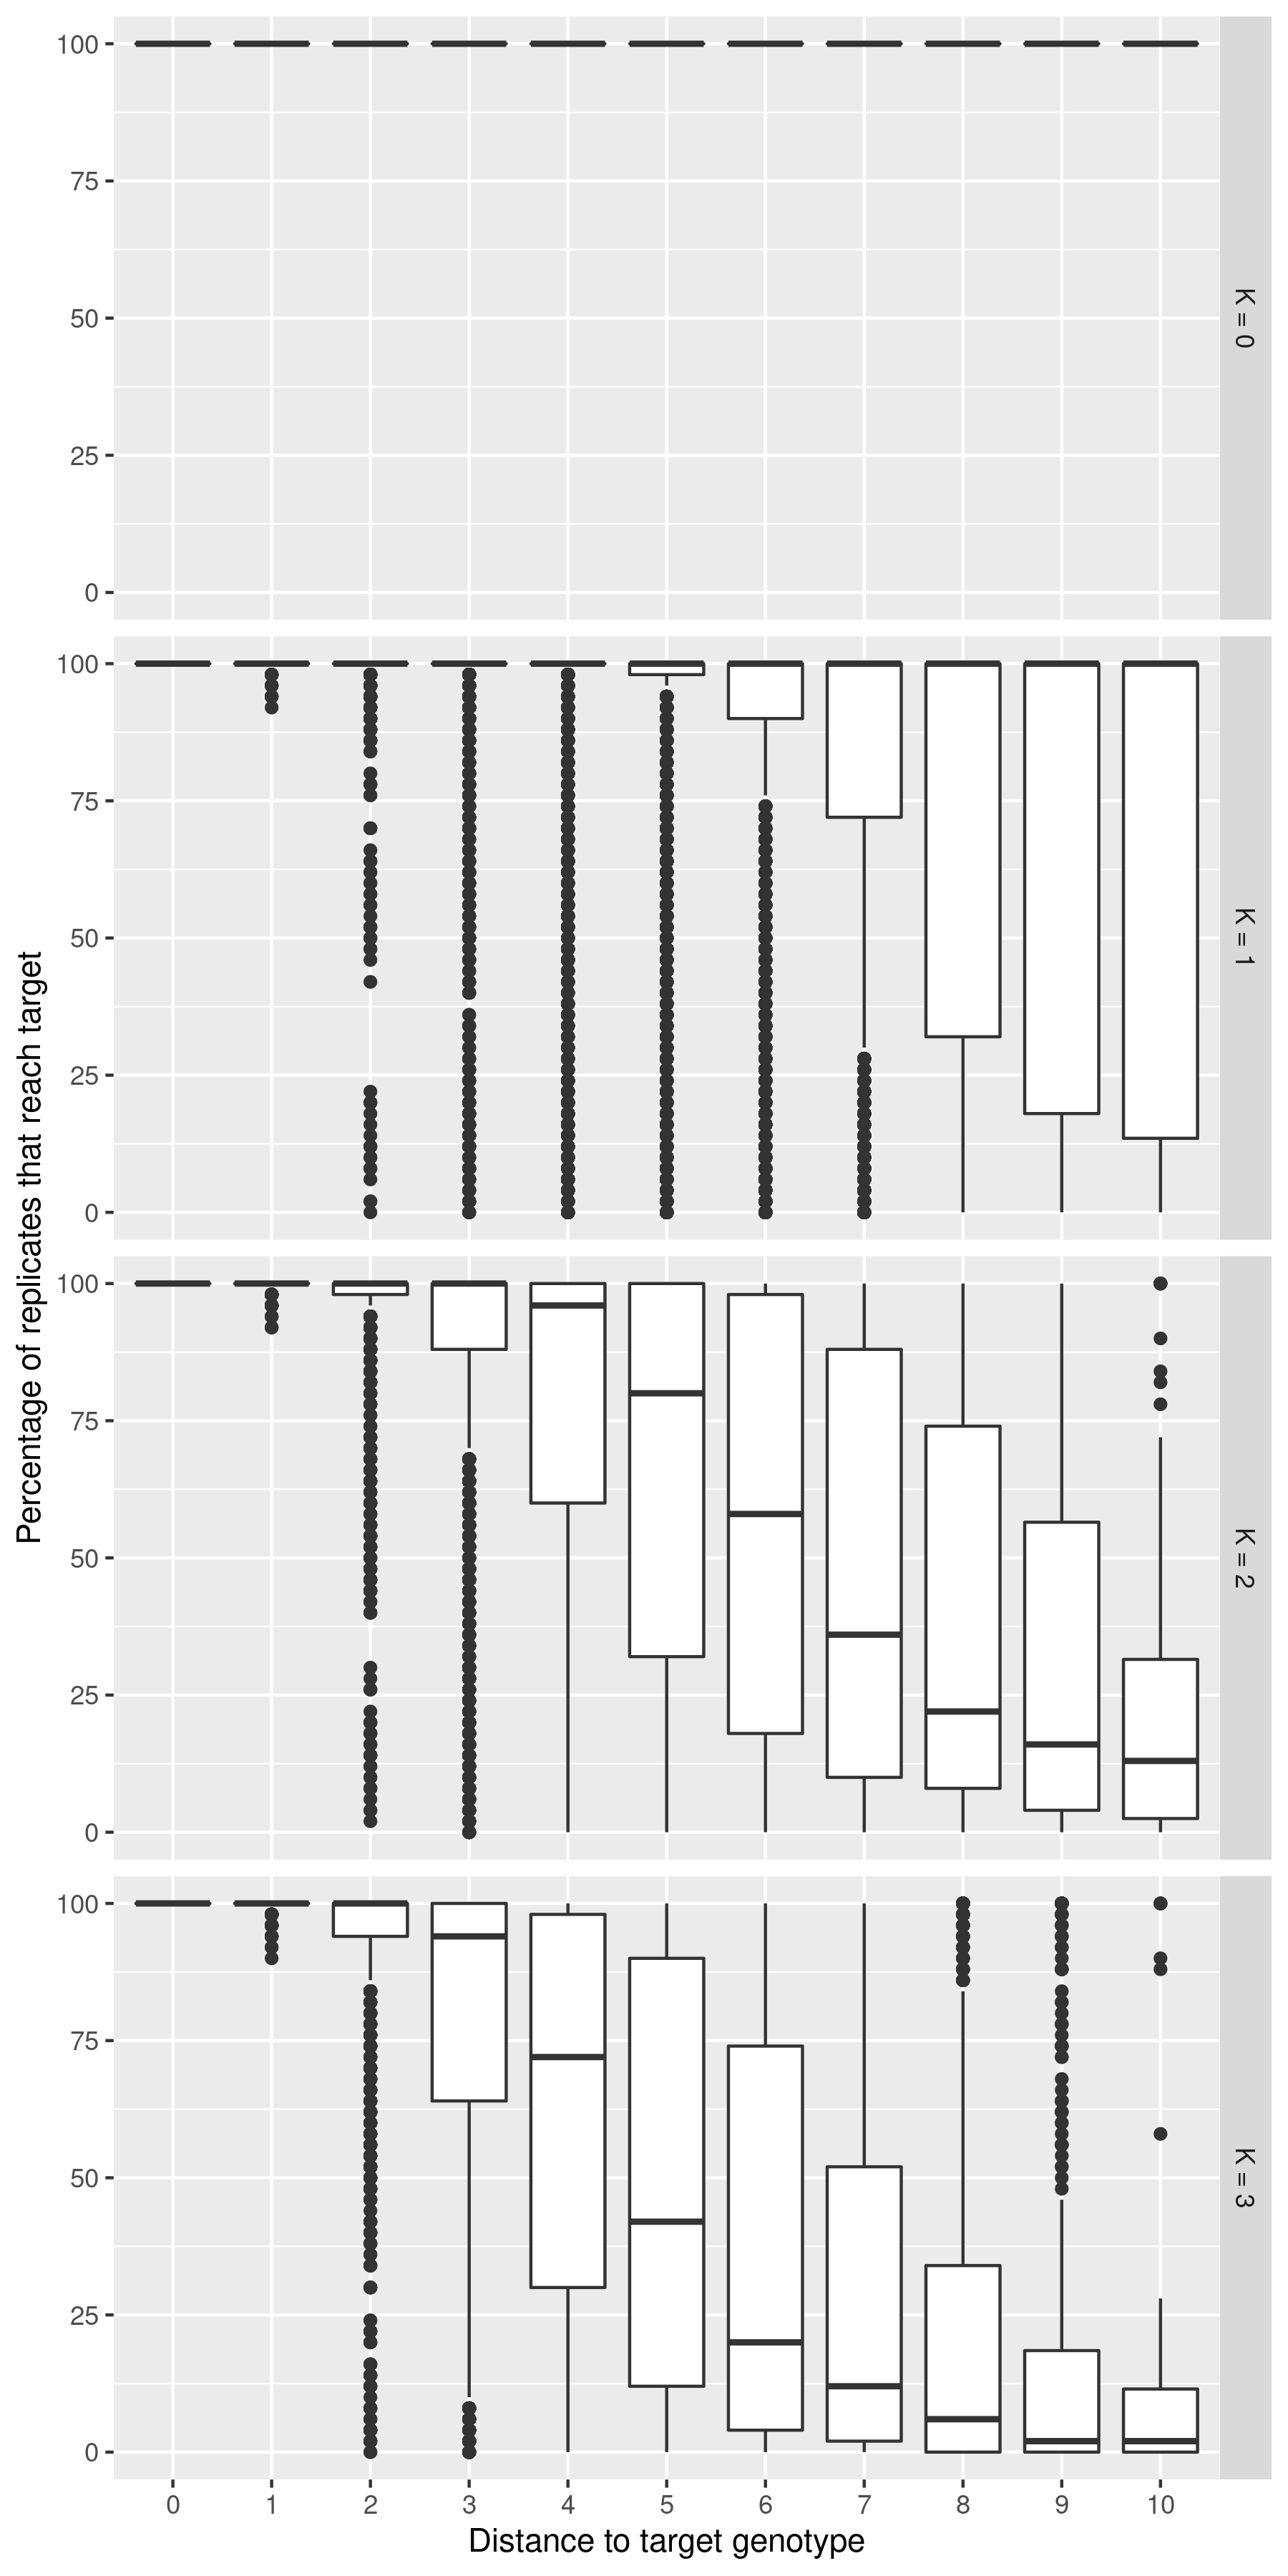
\includegraphics[width=0.6\textwidth]{04_simplified_model/media/potentiation_by_distance_boxplots.png}
    \caption{
        Boxplots showing the potentiation of genotypes at a given distance away from the global optimum. 
        Rows show the various $K$ values, and each boxplot shows all genotypes at that distance for all 50 landscapes for that $K$ value. 
    }
    \label{fig:simplified_model:distance_boxplots}
\end{figure}

Finally, Figure \ref{fig:simplified_model:distance_boxplots} shows how potentiation changes as we vary $K$ and look at the distance from a genotype to the target trait.
As we have already seen, $K = 0$ is a single hill and thus all genotypes are fully potentiated. 
Starting at $K=1$, we see that while the median potentiation stays consistently high, the lowest quartile decreases as distance from the target increases. 
At $K=2$, we see the whole distribution of potentiation shift to lower values as distance increases, with very few points at the maximum distance having high potentiation. 
This trend continues into $K = 3$, becoming more pronounced. 
Overall, Figure \ref{fig:simplified_model:distance_boxplots} meets my expectations. 
In the simpler landscapes, most genotypes have high potentiation, but as the landscapes become more rugged we see potentiation fall faster as we increase the distance to the target. 

While these data are only a shallow glance into potentiation in NK landscapes, they provide reassurance that the system is worthy of examination. % looking into.
When performing the work in earnest, I will be analyzing landscapes with higher values of $N$ and $K$. %, and performing deeper analyses by looking at aspects such as the basins of attraction to the target.
Additionally, I will be looking at the lineages of semi-potentiated genotypes, allowing me to compare the potentiation measures that will be recorded in Chapter \ref{chap:replaying_associative_learning}. 
This brief glimpse reveals promise in the system; hopefully this promise holds true and NK landscapes can help us delve further into potentiation. 